\documentclass[11pt,a4paper]{report}
\usepackage[utf8]{inputenc}
\usepackage[T1]{fontenc}
\usepackage{amsmath,amssymb,amsfonts}
\usepackage{graphicx}
\usepackage{booktabs}
\usepackage{longtable}
\usepackage{hyperref}
\usepackage{listings}
\usepackage{xcolor}
\usepackage{tikz}
\usepackage{geometry}
\usepackage{fancyhdr}
\usepackage{titlesec}
\usepackage{caption}
\usepackage{subcaption}
\usepackage{enumitem}
\usepackage{algorithm}
\usepackage{algpseudocode}
\usepackage{mdframed}
\usepackage{siunitx}
\usepackage{pifont}

\newcommand{\cmark}{\ding{51}}
\newcommand{\xmark}{\ding{55}}

\geometry{margin=2.5cm}
\hypersetup{colorlinks=true,linkcolor=blue,citecolor=blue,urlcolor=blue}

\definecolor{codebg}{RGB}{248,248,248}
\definecolor{codeframe}{RGB}{200,200,200}
\definecolor{warningbg}{RGB}{255,243,205}
\definecolor{warningframe}{RGB}{255,234,167}
\definecolor{infobg}{RGB}{209,236,241}
\definecolor{infoframe}{RGB}{190,230,239}
\definecolor{decisionbg}{RGB}{212,237,218}
\definecolor{decisionframe}{RGB}{195,230,203}

\lstset{
    backgroundcolor=\color{codebg},
    frame=single,
    rulecolor=\color{codeframe},
    basicstyle=\ttfamily\small,
    breaklines=true,
    showstringspaces=false
}

\newmdenv[backgroundcolor=warningbg,linewidth=0.5pt,linecolor=warningframe,roundcorner=3pt,innertopmargin=5pt,innerbottommargin=5pt,innerleftmargin=10pt,innerrightmargin=10pt]{warningbox}
\newmdenv[backgroundcolor=infobg,linewidth=0.5pt,linecolor=infoframe,roundcorner=3pt,innertopmargin=5pt,innerbottommargin=5pt,innerleftmargin=10pt,innerrightmargin=10pt]{infobox}
\newmdenv[backgroundcolor=decisionbg,linewidth=0.5pt,linecolor=decisionframe,roundcorner=3pt,innertopmargin=5pt,innerbottommargin=5pt,innerleftmargin=10pt,innerrightmargin=10pt]{decisionbox}

\title{\textbf{Safe Deep RL for 1v1 Pursuit-Evasion}\\
\large A Comprehensive Project Reference Manual}
\author{Project: safe-rl-pe}
\date{May 2026}

\begin{document}

\maketitle
\tableofcontents
\newpage

%%%%%%%%%%%%%%%%%%%%%%%%%%%%%%%%%%%%%%%%%%%%%%%%%%%%%%%%%%%%%%%%%%%%%%%%%%%%%%%%
\chapter{Introduction}
\label{chap:intro}

\section{What is This Project?}

This project builds a simulation and training framework for \textbf{1v1 pursuit-evasion games} using \textbf{deep reinforcement learning} with \textbf{safety guarantees}. The goal is to train two agents---a pursuer and an evader---to play optimally against each other in a physically realistic environment with partial observability.

\subsection{The Core Question}

Can we train two robots (one chasing, one escaping) to play a near-optimal game of cat-and-mouse using only reinforcement learning, when each robot has limited sensing and must obey physical constraints?

\subsection{Why This Matters}

Pursuit-evasion appears in many real-world scenarios:
\begin{itemize}
    \item \textbf{Search and rescue:} A drone (pursuer) searching for a lost hiker (evader)
    \item \textbf{Security:} A patrol robot intercepting an intruder
    \item \textbf{Autonomous driving:} Collision avoidance as a game between vehicles
    \item \textbf{Military:} Target tracking and evasion tactics
\end{itemize}

Traditional approaches use hand-crafted heuristics or model-based planning. This project asks: \textit{Can the agents learn optimal strategies entirely from experience?}

\section{What Makes It Hard?}

\subsection{Challenge 1: Adversarial Dynamics}
Unlike standard RL where an agent learns against a fixed environment, here both agents are learning \emph{simultaneously} and \emph{against each other}. This is a two-player zero-sum game:
\begin{itemize}
    \item If the pursuer gets better, the evader must adapt or lose
    \item If the evader finds a new escape strategy, the pursuer must counter it
    \item This creates an ``arms race'' that can easily collapse
\end{itemize}

\subsection{Challenge 2: Partial Observability}
Real robots cannot see everything. They have:
\begin{itemize}
    \item Limited field of view (FOV) --- e.g., \SI{90}{\degree} camera
    \item Sensing range limits --- cannot see across the entire arena
    \item Occlusion --- obstacles block line of sight
\end{itemize}
Training under partial observability is much harder than full observability because the agent must infer hidden state and plan under uncertainty.

\subsection{Challenge 3: Physical Constraints}
Robots are not point masses. They have:
\begin{itemize}
    \item \textbf{Nonholonomic constraints:} Differential-drive robots cannot move sideways
    \item \textbf{Speed limits:} Maximum linear and angular velocities
    \item \textbf{Collision avoidance:} Must not hit obstacles or walls
\end{itemize}

\subsection{Challenge 4: Safety}
Learned policies can be unpredictable. We want \textbf{hard safety guarantees} that the robot will never violate constraints (e.g., never crash into a wall), even if the learned policy suggests it.

\section{Project Overview}

\begin{table}[h]
\centering
\caption{Project Phases}
\label{tab:phases}
\begin{tabular}{@{}lll@{}}
\toprule
\textbf{Phase} \& \textbf{Focus} \& \textbf{Status} \\
\midrule
Phase 1 \& Core simulation, environment, baselines \& Complete \\
Phase 2 \& Safety integration (CBF, Beta policy) \& Complete \\
Phase 2.5 \& Differentiable QP / BarrierNet experiment \& Complete (abandoned) \\
Phase 3 \& Partial observability + self-play \& Active \\
Phase 4 \& Sim-to-real transfer \& Not started \\
Phase 5 \& Analysis, publication (CoRL 2026) \& In progress \\
\bottomrule
\end{tabular}
\end{table}

\textbf{Project stats:} 75+ documented experimental sessions (S1--S75), 754 unit tests, 36 papers reviewed, 50+ training runs, 2 RTX 5090 GPUs.

%%%%%%%%%%%%%%%%%%%%%%%%%%%%%%%%%%%%%%%%%%%%%%%%%%%%%%%%%%%%%%%%%%%%%%%%%%%%%%%%
\chapter{Mathematical Preliminaries}
\label{chap:math}

This chapter establishes the formal foundations upon which the entire project rests. We define Markov Decision Processes, Partially Observable MDPs, differential games, and Nash equilibrium --- the mathematical language of pursuit-evasion.

\section{Markov Decision Processes}

\subsection{Definition}

A \textbf{Markov Decision Process} (MDP) is a tuple $\mathcal{M} = (\mathcal{S}, \mathcal{A}, \mathcal{T}, \mathcal{R}, \gamma)$ where:
\begin{itemize}
    \item $\mathcal{S}$ is the state space
    \item $\mathcal{A}$ is the action space
    \item $\mathcal{T}: \mathcal{S} \times \mathcal{A} \times \mathcal{S} \to [0,1]$ is the transition probability $p(s' | s, a)$
    \item $\mathcal{R}: \mathcal{S} \times \mathcal{A} \to \mathbb{R}$ is the reward function
    \item $\gamma \in [0,1)$ is the discount factor
\end{itemize}

\subsection{Policy and Value Functions}

A \textbf{stationary policy} $\pi: \mathcal{S} \times \mathcal{A} \to [0,1]$ specifies the probability of taking action $a$ in state $s$. The \textbf{state-value function} is:
\begin{equation}
    V^\pi(s) = \mathbb{E}_{\pi}\left[ \sum_{t=0}^{\infty} \gamma^t r(s_t, a_t) \,\middle|\, s_0 = s \right]
\end{equation}

The \textbf{action-value function} (Q-function) is:
\begin{equation}
    Q^\pi(s,a) = \mathbb{E}_{\pi}\left[ \sum_{t=0}^{\infty} \gamma^t r(s_t, a_t) \,\middle|\, s_0 = s, a_0 = a \right]
\end{equation}

They satisfy the \textbf{Bellman equation}:
\begin{equation}
    Q^\pi(s,a) = \mathcal{R}(s,a) + \gamma \mathbb{E}_{s' \sim \mathcal{T}(\cdot|s,a)}\left[ V^\pi(s') \right]
\end{equation}

\subsection{Optimal Policy}

The \textbf{optimal Q-function} $Q^*(s,a) = \max_\pi Q^\pi(s,a)$ satisfies the Bellman optimality equation:
\begin{equation}
    Q^*(s,a) = \mathcal{R}(s,a) + \gamma \mathbb{E}_{s' \sim \mathcal{T}(\cdot|s,a)}\left[ \max_{a'} Q^*(s', a') \right]
\end{equation}

An \textbf{optimal policy} $\pi^*$ is any policy that is greedy with respect to $Q^*$:
\begin{equation}
    \pi^*(a|s) = \begin{cases} 1 & \text{if } a \in \arg\max_{a'} Q^*(s,a') \\ 0 & \text{otherwise} \end{cases}
\end{equation}

\section{Partially Observable Markov Decision Processes}

\subsection{Definition}

In pursuit-evasion, agents do not observe the full state. We model this as a \textbf{POMDP}: $\mathcal{P} = (\mathcal{S}, \mathcal{A}, \mathcal{O}, \mathcal{T}, \mathcal{Z}, \mathcal{R}, \gamma)$ where:
\begin{itemize}
    \item $\mathcal{S}, \mathcal{A}, \mathcal{T}, \mathcal{R}, \gamma$ are as in the MDP
    \item $\mathcal{O}$ is the observation space
    \item $\mathcal{Z}: \mathcal{S} \times \mathcal{A} \times \mathcal{O} \to [0,1]$ is the observation probability $p(o | s', a)$
\end{itemize}

\subsection{Belief States}

Since the true state is unknown, the agent maintains a \textbf{belief} $b(s) = p(s | h_t)$ where $h_t = (a_0, o_1, a_1, o_2, \ldots, a_{t-1}, o_t)$ is the history. Belief updates follow Bayes' rule:
\begin{equation}
    b'(s') = \eta \, \mathcal{Z}(o | s', a) \sum_{s \in \mathcal{S}} \mathcal{T}(s' | s, a) b(s)
\end{equation}
where $\eta$ is a normalizing constant.

\begin{warningbox}
\textbf{The curse of history:} The belief space is continuous and infinite-dimensional. Exact POMDP solutions are computationally intractable for our problem. This motivates using deep RL to learn approximate policies directly from observations.
\end{warningbox}

\subsection{Information State}

An alternative to beliefs is the \textbf{information state} or \textbf{history} representation: train a recurrent policy $\pi(a_t | o_t, h_{t-1})$ where $h_t = f(h_{t-1}, o_t, a_t)$ is encoded by an LSTM or GRU. We abandoned this approach (RecurrentPPO) because the additional complexity overwhelmed the self-play task.

\section{Game Theory: Two-Player Zero-Sum Games}

\subsection{Normal-Form Games}

A two-player game in normal form is defined by strategy sets $\mathcal{X}, \mathcal{Y}$ and a \textbf{payoff matrix} $A \in \mathbb{R}^{|\mathcal{X}| \times |\mathcal{Y}|}$. Player 1 (maximizer) chooses $x \in \mathcal{X}$, Player 2 (minimizer) chooses $y \in \mathcal{Y}$. The payoff to Player 1 is $x^\top A y$.

\subsection{Zero-Sum Property}

Pursuit-evasion is \textbf{zero-sum}: the pursuer's gain is the evader's loss. If the pursuer wins (capture), the pursuer gets $+100$ and the evader gets $-100$. The sum is always zero.

\subsection{Minimax Theorem (von Neumann, 1928)}

For finite zero-sum games, there exists a \textbf{game value} $v$ such that:
\begin{equation}
    \max_{x \in \Delta(\mathcal{X})} \min_{y \in \Delta(\mathcal{Y})} x^\top A y = \min_{y \in \Delta(\mathcal{Y})} \max_{x \in \Delta(\mathcal{X})} x^\top A y = v
\end{equation}
where $\Delta(\cdot)$ denotes the set of probability distributions (mixed strategies).

\section{Nash Equilibrium}

\subsection{Definition}

A \textbf{Nash equilibrium} (NE) is a strategy pair $(\pi^*_P, \pi^*_E)$ such that neither player can improve their expected payoff by unilaterally changing their strategy:
\begin{align}
    \mathbb{E}[R_P(\pi^*_P, \pi^*_E)] &\geq \mathbb{E}[R_P(\pi_P, \pi^*_E)] \quad \forall \pi_P \\
    \mathbb{E}[R_E(\pi^*_P, \pi^*_E)] &\geq \mathbb{E}[R_E(\pi^*_P, \pi_E)] \quad \forall \pi_E
\end{align}

In zero-sum games, every NE yields the same game value (the \textbf{minimax value}).

\subsection{Epsilon-Nash Equilibrium}

In practice, we settle for an $\varepsilon$-NE where no player can gain more than $\varepsilon$ by deviating:
\begin{equation}
    \mathbb{E}[R_P(\pi^*_P, \pi^*_E)] \geq \max_{\pi_P} \mathbb{E}[R_P(\pi_P, \pi^*_E)] - \varepsilon
\end{equation}

Our convergence criterion ($|\text{CR} - 0.5| < 0.1$) is a heuristic for detecting approximate NE in this adversarial setting.

\subsection{Convergence in Self-Play}

\textbf{Fictitious Play} converges to NE in two-player zero-sum games. However, with function approximation (neural networks) and non-stationary opponents, convergence is not guaranteed. Our alternating freeze protocol is an empirical method to encourage convergence.

\section{Differential Games}

\subsection{Definition}

A \textbf{differential game} extends game theory to continuous-time dynamical systems. The state evolves according to:
\begin{equation}
    \dot{x} = f(x, u_P, u_E)
\end{equation}
where $x \in \mathbb{R}^n$ is the state, $u_P \in \mathcal{U}_P$ and $u_E \in \mathcal{U}_E$ are the players' controls.

\subsection{Isaacs' Equation}

For zero-sum differential games with value function $V(x)$, the \textbf{Hamilton-Jacobi-Isaacs} (HJI) equation is:
\begin{equation}
    \min_{u_E} \max_{u_P} \left[ \nabla V(x)^\top f(x, u_P, u_E) + \ell(x, u_P, u_E) \right] = 0
\end{equation}
where $\ell$ is the running cost. This is the continuous-time analog of the Bellman optimality equation.

\begin{infobox}
\textbf{Theoretical background:} HJI reachability (Theme 5 in literature review) computes the "capture set" --- the set of initial states from which the pursuer can guarantee capture. \textbf{Note:} Our safety approach uses CBF-QP filtering, not HJI reachability. HJI is computationally intractable for our problem dimension.
\end{infobox}

%%%%%%%%%%%%%%%%%%%%%%%%%%%%%%%%%%%%%%%%%%%%%%%%%%%%%%%%%%%%%%%%%%%%%%%%%%%%%%%%
\chapter{Background and Literature Review}
\label{chap:literature}

\section{The Research Landscape}

We reviewed \textbf{36 original papers} plus 15 supplementary papers across 6 major themes. This chapter summarizes what exists, what works, and---most importantly---\textbf{what gap our project fills}.

\subsection{Six Themes}

\begin{table}[h]
\centering
\caption{Literature Themes}
\label{tab:themes}
\begin{tabular}{@{}p{4cm}p{2.5cm}p{6cm}@{}}
\toprule
\textbf{Theme} \& \textbf{Papers} \& \textbf{Key Question} \\
\midrule
Direct 1v1 PE with Deep RL \& [01,02,08,12--15,22,34] \& Can RL learn effective pursuit-evasion policies? \\
Safety-Constrained RL \& [03,05,06,10,13,14,16,27,28,30] \& How to guarantee safety during learning? \\
Self-Play \& MARL \& [04,11,18,19,20,37] \& How to train adversarial agents to convergence? \\
Sim-to-Real Transfer \& [02,07,08,18,22] \& Do learned policies work on real robots? \\
HJ Reachability \& Neural \& [21--25,31,35] \& Can we compute game-optimal solutions? \\
Novel Architectures \& [17,32,34] \& What network structures help? \\
\bottomrule
\end{tabular}
\end{table}

\section{Theme 1: Direct 1v1 Pursuit-Evasion with Deep RL}

\subsection{Problem Formulation}

The direct pursuit-evasion RL problem is formulated as a two-player Markov game $\mathcal{G} = (\mathcal{S}, \mathcal{A}_P, \mathcal{A}_E, \mathcal{T}, \mathcal{R}_P, \mathcal{R}_E, \gamma)$. Both players observe (partially) the same state and take simultaneous actions. The key challenge is the \textbf{non-stationarity}: as one agent's policy changes, the effective environment for the other changes.

\subsection{State of the Art: Gonultas \& Isler [02]}

\textbf{Title:} ``Learning to Play Pursuit-Evasion Games with Limited Information''

\textbf{Methodology:}
\begin{itemize}
    \item \textbf{Environment:} Car-like robots in ROS/Gazebo simulation, F1TENTH and JetRacer platforms for real-world deployment
    \item \textbf{Observation:} RGB camera images + LiDAR scans; opponent position inferred via \textbf{Bidirectional Mixture Density Network (BiMDN)} --- a learned belief encoder that outputs a mixture of Gaussians for opponent position
    \item \textbf{Training:} \textbf{MADDPG} (Multi-Agent Deep Deterministic Policy Gradient) with curriculum learning: start with easy opponent trajectories, progressively increase difficulty
    \item \textbf{Action space:} Continuous steering and throttle
\end{itemize}

\textbf{Results:}
\begin{itemize}
    \item BiMDN improved capture rate by 16\% over raw observations
    \item Real-world transfer showed performance degradation (sim-to-real gap)
    \item Convergence to stable policies demonstrated
\end{itemize}

\textbf{Limitations:}
\begin{itemize}
    \item No safety guarantees --- agents could collide with obstacles
    \item BiMDN requires opponent to be occasionally visible for belief updates
    \item Full observability of obstacles assumed
    \item No formal Nash equilibrium convergence proof
\end{itemize}

\textbf{Our improvement:} We abandoned BiMDN after it failed Gate 1 (could not predict opponent position when completely unobserved). Our visibility reward + search staleness approach provides a denser learning signal without requiring accurate belief states.

\subsection{AMS-DRL: Adversarial Multi-Stage DRL [18]}

\textbf{Title:} ``AMS-DRL: Adversarial Multi-Stage Deep Reinforcement Learning for Pursuit-Evasion''

\textbf{Methodology:}
\begin{itemize}
    \item \textbf{Multi-pursuer} setting: $N$ pursuers vs 1 evader
    \item \textbf{Staged asynchronous alternation:} Train pursuers while evader is frozen, then train evader while pursuers are frozen
    \item \textbf{Mathematical guarantee:} Proves that under certain conditions (Lipschitz continuity, bounded rewards), the alternation converges to a Nash equilibrium
    \item \textbf{Real deployment:} Tello Edu drones
\end{itemize}

\textbf{Key Theoretical Result:}
Let $\pi_P^t$ and $\pi_E^t$ be the policies at stage $t$. If the policy updates satisfy:
\begin{equation}
    \|\pi^{t+1} - \pi^t\| \leq \frac{\epsilon}{L}
\end{equation}
where $L$ is the Lipschitz constant of the value function, then the sequence converges to an $\epsilon$-NE.

\textbf{Limitations:}
\begin{itemize}
    \item \textbf{Omni-directional sensing:} Drones have 360° cameras --- no partial observability challenge
    \item \textbf{Holonomic dynamics:} Drones can move in any direction --- no differential-drive constraints
    \item No safety filter or collision avoidance guarantees
    \item Multi-pursuer setting does not directly translate to our 1v1 problem
\end{itemize}

\textbf{Our improvement:} We adopted their staged alternation concept but adapted it for partial observability and nonholonomic ground robots. Our forced periodic switch mechanism addresses the ``freeze-sticking'' problem not covered in their theory.

\subsection{MADR: Model-Based Adversarial PE [22]}

\textbf{Title:} ``Game-Optimal Pursuit-Evasion on TurtleBots''

\textbf{Methodology:}
\begin{itemize}
    \item \textbf{DeepReach:} Neural network approximation of Hamilton-Jacobi reachability
    \item \textbf{Adversarial MPC:} Model Predictive Control with game-theoretic cost
    \item \textbf{Safety:} 98.9\% collision-free rate via MPC constraints
    \item \textbf{Platform:} TurtleBot3 in 10x10m arena with obstacles
\end{itemize}

\textbf{Results:}
\begin{itemize}
    \item 500+ second engagements (very long episodes)
    \item Game-optimal trajectories computed in real-time
    \item Robust to model mismatch
\end{itemize}

\textbf{Limitations:}
\begin{itemize}
    \item \textbf{Requires known dynamics model:} The MPC needs accurate system identification
    \item \textbf{Not model-free:} Cannot learn from raw experience
    \item \textbf{Computational cost:} DeepReach training takes days on GPU clusters
    \item Safety is embedded in MPC, not a learned filter --- harder to certify
\end{itemize}

\textbf{Our improvement:} We are fully model-free. Our safety filter (CBF-QP) is modular and can be applied to any learned policy without retraining.

\subsection{SHADOW: Information-Aware PE [34]}

\textbf{Title:} ``SHADOW: Information-Aware Adversarial Multi-Agent Reinforcement Learning''

\textbf{Methodology:}
\begin{itemize}
    \item \textbf{Three-module architecture:} Navigation Module (TD3 + LSTM), Query Decision Module (PPO + LSTM), Opponent Modeling Module
    \item \textbf{Opponent modeling:} Dedicated module that predicts opponent actions with uncertainty quantification
    \item \textbf{Dual RL algorithms:} TD3 for navigation decisions, PPO for communication/query decisions
\end{itemize}

\textbf{Results:}
\begin{itemize}
    \item 62\% win rate vs 18.4\% baseline when opponent model is accurate
    \item Robust to partial observability via belief state encoding
\end{itemize}

\textbf{Limitations:}
\begin{itemize}
    \item No safety guarantees
    \item No self-play convergence proof --- single fixed opponent
    \item Complex architecture with many hyperparameters
\end{itemize}

\section{Theme 2: Safety-Constrained Reinforcement Learning}

\subsection{Safety in Control Theory}

Safety in dynamical systems is formalized using \textbf{set invariance}. A set $\mathcal{C} \subset \mathbb{R}^n$ is called \textbf{forward invariant} under dynamics $\dot{x} = f(x,u)$ if:
\begin{equation}
    x(0) \in \mathcal{C} \implies x(t) \in \mathcal{C} \quad \forall t \geq 0
\end{equation}

The \textbf{safe set} $\mathcal{C}$ is typically defined as the zero-superlevel set of a function $h: \mathbb{R}^n \to \mathbb{R}$:
\begin{equation}
    \mathcal{C} = \{x \in \mathbb{R}^n : h(x) \geq 0\}
\end{equation}

For example, obstacle avoidance: $h(x) = \|x - x_{\text{obs}}\| - r_{\text{obs}}$ where $r_{\text{obs}}$ is the obstacle radius.

\subsection{Control Barrier Functions (CBF)}

\subsubsection{Definition}
A function $h: \mathbb{R}^n \to \mathbb{R}$ is a \textbf{valid Control Barrier Function} for the safe set $\mathcal{C}$ if there exists an extended class-$\mathcal{K}_\infty$ function $\alpha$ such that:
\begin{equation}
    \sup_{u \in \mathcal{U}} \left[ \mathcal{L}_f h(x) + \mathcal{L}_g h(x) u + \alpha(h(x)) \right] \geq 0 \quad \forall x \in \mathcal{C}
\end{equation}
where $\mathcal{L}_f h = \nabla h \cdot f$ and $\mathcal{L}_g h = \nabla h \cdot g$ are Lie derivatives, assuming control-affine dynamics $\dot{x} = f(x) + g(x)u$.

\subsubsection{Safety Guarantee (Theorem)}
If $h$ is a valid CBF and the QP:
\begin{equation}
    \begin{aligned}
        \min_{u} \quad & \|u - u_{\text{RL}}\|^2 \\
        \text{s.t.} \quad & \mathcal{L}_f h(x) + \mathcal{L}_g h(x) u + \alpha(h(x)) \geq 0
    \end{aligned}
\end{equation}
is feasible, then the safe set $\mathcal{C}$ is forward invariant. The robot will never leave the safe set.

\subsubsection{Critical Implementation Issue: Mixed Relative Degree}

For nonholonomic robots with dynamics:
\begin{align}
    \dot{x} &= v \cos(\theta) \\
    \dot{y} &= v \sin(\theta) \\
    \dot{\theta} &= \omega
\end{align}

The position $(x,y)$ has \textbf{relative degree 2} with respect to the control $\omega$ (needs two derivatives to appear), but the heading $\theta$ has \textbf{relative degree 1}. This \textbf{mixed relative degree} makes standard CBFs fail.

\textbf{Solution: Virtual Control Point (VCP) [N12]}

Define a point at distance $d$ ahead of the robot:
\begin{equation}
    x_{\text{vcp}} = x + d \cos(\theta), \quad y_{\text{vcp}} = y + d \sin(\theta)
\end{equation}

The VCP has relative degree 1 with respect to $\omega$:
\begin{equation}
    \dot{x}_{\text{vcp}} = v \cos(\theta) - d \omega \sin(\theta)
\end{equation}

Applying the CBF constraint at the VCP instead of the center ensures steering (not just braking) can satisfy safety constraints.

\subsection{CBF Safety Filter (QP) [05, 06]}

\textbf{Papers:} ``Control Barrier Functions for Systems with High Relative Degree'' [05], ``End-to-End Safe Reinforcement Learning'' [06]

\textbf{Method:} After RL proposes $u_{\text{RL}}$, solve a Quadratic Program to find the closest safe action:
\begin{equation}
    \begin{aligned}
        \min_{u, \delta} \quad & \|u - u_{\text{RL}}\|^2 + \lambda \|\delta\|^2 \\
        \text{s.t.} \quad & \text{Wall CBF: } \nabla h_w \cdot f(x,u) + \alpha(h_w(x)) \geq -\delta_w \\
        & \text{Obstacle CBF: } \nabla h_o \cdot f(x,u) + \alpha(h_o(x)) \geq -\delta_o \\
        & u \in \mathcal{U}
    \end{aligned}
\end{equation}
where $\delta$ are slack variables that allow constraint relaxation when infeasible.

\textbf{Pros:} Hard safety guarantee, modular (works with any RL algorithm), provably correct.

\textbf{Cons:} QP must be solved at every control step (\textasciitilde 1ms on modern hardware), may be infeasible (no safe action exists), can block exploration if too aggressive.

\subsection{CBF-Constrained Policy [16]}

\textbf{Paper:} ``Safe Reinforcement Learning via Control Barrier Functions'' (Suttle et al.)

\textbf{Breakthrough:} First approach to achieve \textbf{both convergence guarantees AND hard safety constraints} simultaneously.

\textbf{Method:}
\begin{itemize}
    \item Policy outputs parameters of a \textbf{Beta distribution} (naturally bounded in $[0,1]$)
    \item CBF constraints are enforced during policy optimization via Lagrangian relaxation
    \item Provably converges to a safe policy under standard RL assumptions
\end{itemize}

\textbf{Key Theoretical Result:}
If the policy class is sufficiently expressive and the CBF is valid, the algorithm converges to a policy that:
\begin{enumerate}
    \item Satisfies the CBF safety constraint with probability 1
    \item Achieves reward within $\epsilon$ of the optimal safe policy
\end{enumerate}

\textbf{Limitations:}
\begin{itemize}
    \item Requires accurate dynamics model for CBF computation
    \item Beta policy limits action distribution flexibility
    \item No partial observability handling
\end{itemize}

\section{Theme 3: Self-Play and Multi-Agent RL}

\subsection{Training Paradigms: Mathematical Formulation}

\subsubsection{Vanilla Self-Play}
Both agents train simultaneously against each other. At iteration $t$:
\begin{align}
    \pi_P^{t+1} &= \arg\max_{\pi_P} \mathbb{E}[R_P(\pi_P, \pi_E^t)] \\
    \pi_E^{t+1} &= \arg\max_{\pi_E} \mathbb{E}[R_E(\pi_P^t, \pi_E)]
\end{align}

\textbf{Problem:} The environment is non-stationary. The evader's policy changes every iteration, so the pursuer's past experience becomes obsolete. This causes \textbf{strategy cycling}.

\subsubsection{Fictitious Self-Play (FSP)}

Instead of playing against the current opponent, play against the \textbf{average} of all past opponents:
\begin{equation}
    \bar{\pi}^t = \frac{1}{t} \sum_{i=1}^{t} \pi^i
\end{equation}

\textbf{Theorem (Robinson, 1951):} In two-player zero-sum games, fictitious play converges to a Nash equilibrium.

\textbf{In practice:} Computing the average policy is expensive for neural networks. OpenAI Five used an approximate version.

\subsubsection{Policy Space Response Oracles (PSRO)}

\textbf{Used by:} AlphaStar, AlphaZero

Maintain a \textbf{population} of strategies $\Pi = \{\pi_1, \pi_2, \ldots, \pi_N\}$. At each iteration:
\begin{enumerate}
    \item Compute a \textbf{meta-game} payoff matrix $M_{ij} = \mathbb{E}[R(\pi_i, \pi_j)]$
    \item Solve for Nash equilibrium $\sigma^*$ of the meta-game
    \item Train a new best response $\pi_{N+1}$ against the NE mixture $\sum_i \sigma^*_i \pi_i$
    \item Add $\pi_{N+1}$ to the population
\end{enumerate}

\textbf{Theorem:} PSRO converges to a Nash equilibrium of the full game if the best response computation is exact.

\textbf{Limitations:}
\begin{itemize}
    \item Requires evaluating all pairs in the population (expensive)
    \item Best response computation is approximate with neural networks
    \item Population can grow very large
\end{itemize}

\subsubsection{AMS-DRL Staged Alternation [18]}

Train one role while freezing the other. The switch condition is based on performance:
\begin{equation}
    \text{Switch if } |\text{CR} - 0.5| < \epsilon \text{ for } K \text{ consecutive evaluations}
\end{equation}

\textbf{Theoretical guarantee:} Under Lipschitz continuity, staged alternation converges to NE.

\textbf{Practical issue:} What if one agent never reaches the threshold? The frozen agent never trains.

\subsection{Why Self-Play is Hard: Formal Analysis}

\subsubsection{Catastrophic Forgetting}

When agent $A$ trains against opponent $B$, it optimizes $\pi_A$ to beat $\pi_B$. If $B$ then changes to $\pi_B'$, $A$'s policy may lose performance against $\pi_B$.

\textbf{Formalization:} Let $J(\pi_A, \pi_B)$ be the expected return. After training:
\begin{equation}
    J(\pi_A^{\text{new}}, \pi_B') > J(\pi_A^{\text{old}}, \pi_B')
\end{equation}
but potentially:
\begin{equation}
    J(\pi_A^{\text{new}}, \pi_B) \ll J(\pi_A^{\text{old}}, \pi_B)
\end{equation}

\textbf{Our solution:} Opponent pool with PFSP sampling forces the agent to maintain performance against diverse past opponents.

\subsubsection{Non-Transitivity}

Rock-paper-scissors dynamics: $\pi_A$ beats $\pi_B$, $\pi_B$ beats $\pi_C$, but $\pi_C$ beats $\pi_A$.

\textbf{Implication:} There is no single ``best'' policy. The goal is not to find the best policy, but to find a \textbf{Nash equilibrium strategy} that is unexploitable.

\subsubsection{Freeze-Sticking}

If the pursuer consistently wins at CR = 0.64 (just below the threshold), it keeps training while the evader never gets gradient signal.

\textbf{Our solution:} Forced periodic switching every 2M steps ensures both agents get training time regardless of performance.

\section{Theme 4: Sim-to-Real Transfer}

\subsection{The Sim-to-Real Gap}

Transferring policies from simulation to real robots faces several challenges:
\begin{enumerate}
    \item \textbf{Dynamics mismatch:} $f_{\text{sim}}(x,u) \neq f_{\text{real}}(x,u)$
    \item \textbf{Observation noise:} Real sensors have noise not present in simulation
    \item \textbf{Actuator delay:} Real motors have latency
    \item \textbf{Unmodeled physics:} Friction, gear backlash, wheel slip
\end{enumerate}

\subsection{Domain Randomization [07, 08]}

Train with randomized physics parameters:
\begin{equation}
    \theta \sim p(\theta) \quad \text{where } \theta = \{\text{mass, friction, inertia, \ldots}\}
\end{equation}

\textbf{Result:} Policies trained with sufficient randomization transfer without fine-tuning.

\textbf{Limitations:}
\begin{itemize}
    \item Requires wide randomization distribution --- may make training harder
    \item No guarantee that real parameters are in the training distribution
    \item Conservative policies (optimizing worst-case randomization)
\end{itemize}

\subsection{AMS-DRL Real Deployment [18]}

Achieved real drone deployment by:
\begin{enumerate}
    \item Training in simulation with domain randomization
    \item Fine-tuning on real robot for 100 episodes
    \item Using onboard computation (no cloud dependency)
\end{enumerate}

\textbf{Key insight:} The neural network architecture must be small enough for real-time inference on embedded hardware.

\section{Theme 5: Hamilton-Jacobi Reachability}

\subsection{HJI Reachability Basics}

For a differential game with dynamics $\dot{x} = f(x, u_P, u_E)$, the \textbf{backwards reachable tube} $\mathcal{R}(t)$ is the set of initial states from which the pursuer can guarantee capture within time $t$:
\begin{equation}
    \mathcal{R}(t) = \{x_0 : \exists \pi_P \, \forall \pi_E \, \text{s.t. capture within } t\}
\end{equation}

The \textbf{value function} $V(x,t)$ satisfies the HJI equation:
\begin{equation}
    \frac{\partial V}{\partial t} + \min_{u_E} \max_{u_P} \nabla V \cdot f(x, u_P, u_E) = 0
\end{equation}

\subsection{DeepReach [21, 22, 35]}

\textbf{Problem:} Solving HJI on a grid suffers from the ``curse of dimensionality.'' A 10D state space with 100 grid points per dimension requires $100^{10}$ grid points.

\textbf{Solution:} Approximate $V(x,t)$ with a neural network $V_\theta(x,t)$:
\begin{equation}
    \min_\theta \mathbb{E}_{x,t}\left[ \left| \frac{\partial V_\theta}{\partial t} + \min_{u_E} \max_{u_P} \nabla V_\theta \cdot f \right|^2 \right]
\end{equation}

\textbf{Advantages:}
\begin{itemize}
    \item Handles high-dimensional state spaces
    \item Continuous representation (no grid discretization)
    \item Fast query: just one neural network forward pass
\end{itemize}

\textbf{Limitations:}
\begin{itemize}
    \item Requires known dynamics
    \item Training takes days on GPU clusters
    \item No partial observability handling
    \item Hard to incorporate learned opponent behavior
\end{itemize}

\section{Theme 6: Novel Architectures}

\subsection{Multi-Headed Networks [34]}

Separate neural network heads for different information streams:
\begin{equation}
    Q(s,a) = Q_{\text{self}}(s_{\text{self}}, a) + Q_{\text{opp}}(b_{\text{opp}}, a) + Q_{\text{obs}}(o_{\text{obs}}, a)
\end{equation}

\textbf{Advantage:} Each head can specialize. If opponent information is missing, $Q_{\text{opp}}$ can be masked without affecting other heads.

\subsection{Mixture Density Networks (MDN)}

Instead of predicting a single value, predict parameters of a probability distribution:
\begin{equation}
    p(y|x) = \sum_{k=1}^{K} \pi_k(x) \, \mathcal{N}(y; \mu_k(x), \sigma_k(x))
\end{equation}

Used by [02] for opponent position belief encoding. We abandoned this approach (BiMDN) because it failed when the opponent was completely unobserved.

\section{Comprehensive Gap Analysis}

\subsection{The Integration Challenge}

Each theme in the literature addresses a subset of the full problem:
\begin{itemize}
    \item Theme 1 (Direct RL) handles learning but ignores safety and convergence
    \item Theme 2 (Safety) guarantees safety but assumes known dynamics or single-agent setting
    \item Theme 3 (Self-Play) converges in theory but fails under partial observability
    \item Theme 4 (Sim-to-Real) transfers policies but requires the policy to already exist
    \item Theme 5 (HJ Reachability) computes optimal solutions but is computationally intractable
\end{itemize}

\begin{decisionbox}
\textbf{Core Gap:} No existing work combines ALL of the following in a single system:
\begin{enumerate}
    \item \textbf{Safe DRL:} Hard safety constraints via CBF, learned policies
    \item \textbf{Adversarial game:} 1v1 zero-sum pursuit-evasion
    \item \textbf{Ground robots:} Nonholonomic differential-drive dynamics
    \item \textbf{Partial observability:} Realistic FOV + LOS + occlusion
    \item \textbf{Self-play convergence:} Stable co-evolution to Nash equilibrium
    \item \textbf{Model-free:} No need for accurate dynamics model
\end{enumerate}
\end{decisionbox}

\subsection{Why Integration is Non-Trivial}

The naive combination of existing methods fails due to \textbf{negative interactions}:

\begin{enumerate}
    \item \textbf{Safety + Exploration:} Post-hoc CBF filter modifies actions. If the RL policy proposes unsafe actions too often, the filter dominates and the agent cannot explore (our BarrierNet finding: 87.5\% intervention rate, 2\% CR).

    \item \textbf{Self-Play + PO:} Under partial observability, the non-stationarity is amplified. When the evader learns a new hiding strategy, the pursuer cannot see it and gets no learning signal.

    \item \textbf{CBF + Nonholonomic:} Standard CBFs fail for differential-drive robots. The VCP fix is necessary but changes the effective robot geometry.

    \item \textbf{NE Convergence + Function Approximation:} Theoretical guarantees (Fictitious Play, PSRO) assume exact best responses. Neural network approximation breaks these guarantees.
\end{enumerate}

\subsection{Our Position Relative to Competitors}

\begin{table}[h]
\centering
\caption{Competitor Comparison}
\label{tab:competitors}
\begin{tabular}{@{}lccccc@{}}
\toprule
\textbf{Work} \& \textbf{Safe} \& \textbf{PO} \& \textbf{Self-Play} \& \textbf{Ground} \& \textbf{Real} \\
\midrule
Gonultas [02] \& \xmark \& \cmark \& \cmark \& \cmark \& \cmark \\
MADR [22] \& \cmark* \& \cmark \& \xmark \& \cmark \& \cmark \\
AMS-DRL [18] \& \xmark \& \xmark \& \cmark \& \xmark \& \cmark \\
SHADOW [34] \& \xmark \& \cmark \& \xmark \& \cmark \& \xmark \\
\textbf{Our Work} \& \textbf{\cmark} \& \textbf{\cmark} \& \textbf{\cmark} \& \textbf{\cmark} \& \textbf{Planned} \\
\bottomrule
\end{tabular}
\\{\small *MADR uses MPC safety, not learned safety filter}
\end{table}

%%%%%%%%%%%%%%%%%%%%%%%%%%%%%%%%%%%%%%%%%%%%%%%%%%%%%%%%%%%%%%%%%%%%%%%%%%%%%%%%
\chapter{Codebase Architecture}
\label{chap:codebase}

\section{Directory Structure}

\begin{lstlisting}
safe-rl-pe/
|-- agents/              # Neural network architectures
|   |-- bimdn.py        # Bidirectional MDN (failed, documented)
|   |-- encoders.py     # Observation encoders
|   |-- partial_obs_policy.py
|   |-- barriernet_actor.py    # BarrierNet (abandoned)
|   |-- barriernet_ppo.py      # BarrierNet + PPO (abandoned)
|   +-- beta_policy.py  # Beta distribution for bounded actions
|
|-- conf/               # Hydra configuration files
|   |-- algorithm/      # PPO, SAC, RecurrentPPO configs
|   |-- env/            # Environment parameters
|   |-- experiment/     # Experiment definitions
|   |-- safety/         # CBF, DCBF parameters
|   +-- self_play/      # Training protocol configs
|
|-- envs/               # Core environment (Gymnasium)
|   |-- pursuit_evasion_env.py   # Main PE environment
|   |-- observations.py          # Observation builder
|   |-- rewards.py               # Reward computation
|   |-- dynamics.py              # Unicycle physics
|   |-- rendering.py             # Pygame visualization
|   |-- sensors.py               # Lidar / FOV simulation
|   |-- partial_obs_wrapper.py   # LOS/FOV masking
|   |-- dcbf_action_wrapper.py   # Safety filter wrapper
|   |-- search_staleness.py      # Grid-based coverage tracker
|   +-- navigation_env.py        # Cold-start pre-training env
|
|-- safety/             # Safety layer implementations
|   |-- vcp_cbf.py              # Virtual Control Point CBF
|   |-- differentiable_qp.py    # Differentiable QP (BarrierNet)
|   |-- beta_policy.py          # Beta distribution policy
|   |-- safe_beta_policy.py     # CBF-safe Beta policy
|   +-- infeasibility.py        # 3-tier fallback system
|
|-- training/           # Training framework
|   |-- amsdrl.py               # Main AMS-DRL protocol
|   |-- curriculum.py           # Progressive difficulty
|   |-- opponent_pool.py        # PFSP opponent sampling
|   |-- checkpoint_manager.py   # Best-model checkpointing
|   |-- selfplay_callbacks.py   # Health monitoring
|   |-- ewc.py                  # Elastic Weight Consolidation
|   +-- safe_self_play.py       # Safety-aware training
|
|-- scripts/            # Entry points
|   |-- train_amsdrl.py         # Main training script
|   |-- evaluate_comparison.py  # Evaluation
|   |-- visualize_both_learned_gif_gpu.py  # GPU visualization
|   +-- run_ablation.py, run_baselines.py
|
|-- tests/              # Unit tests (700+)
|-- docs/               # Documentation
|-- paper/              # LaTeX paper source
|-- results/            # Experimental outputs
+-- papers/             # Downloaded research papers
\end{lstlisting}

\section{Key Dependencies}

\begin{itemize}
    \item \textbf{Stable Baselines3 (SB3):} PPO, SAC implementations
    \item \textbf{sb3-contrib:} RecurrentPPO (LSTM support, abandoned)
    \item \textbf{PyTorch:} Neural networks, GPU acceleration
    \item \textbf{Gymnasium:} Environment interface
    \item \textbf{Hydra:} Configuration management
    \item \textbf{WandB/TensorBoard:} Experiment tracking
    \item \textbf{qpth:} Differentiable QP solver (BarrierNet)
    \item \textbf{OpenCV/Pygame:} Rendering and visualization
\end{itemize}

\section{Test Suite}

\textbf{700+ tests} across all modules:
\begin{itemize}
    \item Environment tests: observation space, reward computation, collision detection
    \item Safety tests: CBF feasibility, QP correctness, infeasibility handling
    \item Training tests: checkpoint saving, opponent pool, curriculum advancement
    \item Integration tests: end-to-end training runs with small configs
\end{itemize}

Run: \texttt{./venv/bin/python -m pytest tests/ -v}

%%%%%%%%%%%%%%%%%%%%%%%%%%%%%%%%%%%%%%%%%%%%%%%%%%%%%%%%%%%%%%%%%%%%%%%%%%%%%%%%
\chapter{Environment Design}
\label{chap:env}

\section{Formal POMDP Formulation}

The pursuit-evasion environment is formally a \textbf{two-player partially observable Markov game} with safety constraints. We present the full mathematical formulation here.

\subsection{State Space}

The \textbf{full state} $s \in \mathcal{S}$ contains all information needed to evolve the system deterministically:
\begin{equation}
    s = (x_P, y_P, \theta_P, x_E, y_E, \theta_E, v_P, \omega_P, v_E, \omega_E, \mathcal{O}_1, \ldots, \mathcal{O}_K)
\end{equation}
where $\mathcal{O}_i = (x_i, y_i, r_i)$ are the $K$ circular obstacles.

The state space dimension is:
\begin{equation}
    \dim(\mathcal{S}) = 10 + 3K
\end{equation}

For $K=3$ obstacles: $\dim(\mathcal{S}) = 19$.

\subsection{Action Space}

Each agent outputs a continuous action:
\begin{align}
    a_P &= (v_P, \omega_P) \in \mathcal{A}_P = [0, v_{\max}] \times [-\omega_{\max}, \omega_{\max}] \\
    a_E &= (v_E, \omega_E) \in \mathcal{A}_E = [0, v_{\max}] \times [-\omega_{\max}, \omega_{\max}]
\end{align}

\begin{warningbox}
\textbf{Important:} The linear velocity is bounded as $v \in [0, v_{\max}]$, not $[-v_{\max}, v_{\max}]$. Differential-drive robots cannot move backwards --- they must turn around.
\end{warningbox}

\subsection{Transition Dynamics}

The state evolves via Euler integration of the unicycle dynamics with time step $\Delta t = 0.05$ s (20 Hz):
\begin{align}
    x(t+1) &= x(t) + v(t) \cos(\theta(t)) \Delta t \\
    y(t+1) &= y(t) + v(t) \sin(\theta(t)) \Delta t \\
    \theta(t+1) &= \theta(t) + \omega(t) \Delta t
\end{align}

After integration, collision resolution is applied:
\begin{enumerate}
    \item If agent intersects an obstacle or wall, project to the closest valid position
    \item Preserve velocity component tangent to the collision surface
    \item Apply collision penalty
\end{enumerate}

\subsection{Observation Function}

Each agent receives a \textbf{partial observation} $o_i \in \mathcal{O}_i$ generated by the observation function $\mathcal{Z}_i: \mathcal{S} \to \mathcal{O}_i$:
\begin{equation}
    o_i = \mathcal{Z}_i(s)
\end{equation}

The observation function implements:
\begin{enumerate}
    \item \textbf{Self-state:} Direct access to $(x_i, y_i, \theta_i, v_i, \omega_i)$
    \item \textbf{Opponent state:} Masked by visibility --- see Section \ref{sec:visibility}
    \item \textbf{Obstacles:} Direct access to positions of all obstacles
    \item \textbf{Distance/bearing:} Computed from relative positions
\end{enumerate}

\subsection{Reward Function}

The \textbf{joint reward} $R: \mathcal{S} \times \mathcal{A}_P \times \mathcal{A}_E \times \mathcal{S} \to \mathbb{R}^2$ is:
\begin{equation}
    R(s, a_P, a_E, s') = (r_P, r_E)
\end{equation}

With components:
\begin{align}
    r_P &= r_{\text{capture}} \cdot \mathbb{I}[\text{capture}] + r_{\text{collision},P} + r_{\text{vis}} + r_{\text{search}} + r_{\text{dist}} \\
    r_E &= -r_{\text{capture}} \cdot \mathbb{I}[\text{capture}] + r_{\text{collision},E} + r_{\text{survival}} - r_{\text{dist}}
\end{align}

where $r_{\text{dist}}$ is distance-shaping: positive for pursuer when distance decreases, positive for evader when distance increases.

\subsection{Termination Conditions}

An episode terminates when any of:
\begin{enumerate}
    \item \textbf{Capture:} $\|p_P - p_E\| \leq r_{\text{capture}} = 0.5$ m
    \item \textbf{Timeout:} $t \geq T_{\max} = 1200$ steps
    \item \textbf{External:} Environment reset called
\end{enumerate}

\subsection{Information Structure}

This is a \textbf{simultaneous-move} game: both agents select actions without observing the other's action. The information available to each agent is:
\begin{equation}
    I_i(t) = \{o_i(0), a_i(0), o_i(1), a_i(1), \ldots, o_i(t)\}
\end{equation}

Note that agent $i$ does \textbf{not} observe $a_{-i}(t')$ (opponent's actions) or $o_{-i}(t')$ (opponent's observations).

\section{Arena and Physics}

\subsection{Arena}
\begin{itemize}
    \item Size: $20 \times 20$ meters (configurable: 10$\times$10 to 40$\times$40)
    \item Boundaries: Hard walls --- agents cannot leave
    \item Obstacles: 0--3 circular obstacles, random radius (1--3m), random placement
    \item Episode length: 1200 steps max ($\sim$20 seconds at 60Hz)
    \item Capture radius: 0.5m
\end{itemize}

\subsection{Differential-Drive (Unicycle) Dynamics}
Our robots use \textbf{unicycle} dynamics:
\begin{align}
    \dot{x} \&= v \cos(\theta) \\
    \dot{y} \&= v \sin(\theta) \\
    \dot{\theta} \&= \omega
\end{align}
where $v \in [0, 1.0]$ m/s (robots cannot move backwards) and $\omega \in [-2.84, 2.84]$ rad/s.

\begin{infobox}
\textbf{Key constraint:} Differential-drive robots cannot move sideways. They must turn to change direction. This makes pursuit-evasion significantly harder than with omnidirectional (holonomic) robots.
\end{infobox}

\subsection{Collision Resolution}
When agents hit obstacles or walls:
\begin{enumerate}
    \item Project the agent outside the collision geometry (hard constraint)
    \item Preserve tangential velocity component (slide along surface)
    \item Apply penalty reward: $r_{\text{collision}} = -10$
\end{enumerate}

\section{Observation Space}

Each agent receives a \textbf{continuous observation vector} with the following structure:

\begin{table}[h]
\centering
\caption{Observation Vector (Phase 3: Partial Observability + Obstacles)}
\label{tab:obs}
\begin{tabular}{@{}clll@{}}
\toprule
\textbf{Index} \& \textbf{Feature} \& \textbf{Description} \& \textbf{Normalized} \\
\midrule
0 \& $x_{\text{self}}$ \& Own x-position \& $[-1, 1]$ \\
1 \& $y_{\text{self}}$ \& Own y-position \& $[-1, 1]$ \\
2 \& $\theta_{\text{self}}$ \& Own heading \& $[-1, 1]$ \\
3 \& $v_{\text{self}}$ \& Own linear velocity \& $[-1, 1]$ \\
4 \& $\omega_{\text{self}}$ \& Own angular velocity \& $[-1, 1]$ \\
5 \& $x_{\text{opp}}$ \& Opponent x (masked if not visible) \& $[-1, 1]$ or 0 \\
6 \& $y_{\text{opp}}$ \& Opponent y (masked if not visible) \& $[-1, 1]$ or 0 \\
7 \& $\theta_{\text{opp}}$ \& Opponent heading (masked) \& $[-1, 1]$ or 0 \\
8 \& $v_{\text{opp}}$ \& Opponent velocity (masked) \& $[-1, 1]$ or 0 \\
9 \& $\omega_{\text{opp}}$ \& Opponent angular velocity (masked) \& $[-1, 1]$ or 0 \\
10 \& $d_{\text{opp}}$ \& Distance to opponent \& $[0, 1]$ or 0 \\
11 \& $\phi_{\text{opp}}$ \& Bearing to opponent \& $[-1, 1]$ or 0 \\
12 \& $d_{\text{wall},x}$ \& Distance to nearest wall (x) \& $[0, 1]$ \\
13 \& $d_{\text{wall},y}$ \& Distance to nearest wall (y) \& $[0, 1]$ \\
14 \& $\text{los\_visible}$ \& LOS visibility flag \& $\{0, 1\}$ \\
15+ \& $d_{\text{obs}_i}, \phi_{\text{obs}_i}$ \& Obstacle distance and bearing \& $[0, 1], [-1, 1]$ \\
\bottomrule
\end{tabular}
\end{table}

\textbf{Total dimension:} $15 + 2K$ where $K =$ number of obstacle observations (typically $K = 3$ for nearest 3 obstacles, giving 21 dimensions).

\textbf{Masking rule:} If opponent is not visible (outside FOV, outside range, or LOS blocked by obstacle), opponent features (indices 5--11) are set to 0.0. The agent must learn that 0.0 means ``not visible'' rather than ``at origin.''

\section{Sensing and Observability}

\subsection{Sensing Modes Evolution}
We tried multiple sensing modes before finding what works:

\begin{table}[h]
\centering
\caption{Sensing Mode Evolution}
\label{tab:sensing-evolution}
\begin{tabular}{@{}lllll@{}}
\toprule
\textbf{Mode} \& \textbf{Description} \& \textbf{Arena Coverage} \& \textbf{Result} \& \textbf{Status} \\
\midrule
Full obs \& Perfect knowledge \& 100\% \& Upper bound \& Baseline only \\
3m Omni \& 3m radius, all directions \& 2.8\% \& All 8 runs failed \& Abandoned \\
Radius \& Circular radius only \& $\sim$50\% \& Too permissive \& Early experiments \\
LOS \& Line-of-sight only \& Variable \& Intermediate \& Intermediate \\
\textbf{FOV 90$^\circ$/8m} \& \textbf{Wedge + range + LOS} \& \textbf{$\sim$25\%} \& \textbf{Best results} \& \textbf{Primary} \\
\bottomrule
\end{tabular}
\end{table}

\subsection{Combined Masking (Primary Configuration)}
The opponent is visible only if \textbf{ALL} conditions hold:
\begin{enumerate}
    \item Within sensing radius ($d < 8$ m)
    \item Within FOV ($|\phi| < 45^\circ$)
    \item Line-of-sight is not blocked by obstacles
\end{enumerate}

\subsection{Formal Visibility Model}
\label{sec:visibility}

\subsubsection{Distance Check}

Let $p_i = (x_i, y_i)$ be the position of agent $i$. The distance to the opponent is:
\begin{equation}
    d = \|p_i - p_{-i}\| = \sqrt{(x_i - x_{-i})^2 + (y_i - y_{-i})^2}
\end{equation}

The range condition is:
\begin{equation}
    V_{\text{range}} = \mathbb{I}[d \leq r_{\text{sensor}}]
\end{equation}
where $r_{\text{sensor}} = 8$ m and $\mathbb{I}[\cdot]$ is the indicator function.

\subsubsection{Field of View Check}

Let $\theta_i$ be the heading of agent $i$. The relative bearing to the opponent is:
\begin{equation}
    \phi = \text{atan2}(y_{-i} - y_i, x_{-i} - x_i) - \theta_i
\end{equation}

Normalize to $[-\pi, \pi]$:
\begin{equation}
    \phi = \text{mod}(\phi + \pi, 2\pi) - \pi
\end{equation}

The FOV condition is:
\begin{equation}
    V_{\text{fov}} = \mathbb{I}[|\phi| \leq \phi_{\text{fov}}]
\end{equation}
where $\phi_{\text{fov}} = 45^\circ = \pi/4$ rad.

\subsubsection{Line-of-Sight Check}

The line segment from $p_i$ to $p_{-i}$ must not intersect any obstacle. For each obstacle $\mathcal{O}_k = (x_k, y_k, r_k)$:

The distance from the obstacle center to the line segment is:
\begin{equation}
    d_{\text{los},k} = \min_{t \in [0,1]} \|p_i + t(p_{-i} - p_i) - p_k\|
\end{equation}

The LOS condition is:
\begin{equation}
    V_{\text{los}} = \prod_{k=1}^{K} \mathbb{I}[d_{\text{los},k} > r_k]
\end{equation}

\subsubsection{Combined Visibility}

The opponent is visible if:
\begin{equation}
    V = V_{\text{range}} \cdot V_{\text{fov}} \cdot V_{\text{los}}
\end{equation}

\subsubsection{Observation Masking}

If $V = 0$ (not visible), opponent features are set to 0:
\begin{equation}
    o_i[5:12] = \mathbf{0}
\end{equation}

If $V = 1$, opponent features are populated with normalized relative state.

\begin{warningbox}
\textbf{The Zero-Ambiguity Problem:} When $V = 0$, all opponent features are 0.0. This is \textbf{indistinguishable} from the opponent being at the origin with zero velocity. The agent must learn from context (previous observations, elapsed time) that 0.0 means ``not visible.'' This is a key challenge in POMDP learning.
\end{warningbox}

\subsection{Masking Curriculum}
During training, we anneal from full to partial observability:
\begin{equation}
    p_{\text{full\_obs}}(t) = \max\left(0, 1 - \frac{t}{T_{\text{anneal}}}\right)
\end{equation}
where $T_{\text{anneal}} = 5\text{M}$ steps. This gives agents time to learn basic skills before facing full PO.

\begin{infobox}
\textbf{Why curriculum helps:} Starting with full observability lets agents learn basic pursuit/evasion. Gradually removing information forces them to develop robust strategies rather than memorizing.
\end{infobox}

\section{Reward Design}

\subsection{Terminal Rewards}
\begin{itemize}
    \item \textbf{Capture:} Pursuer gets $+100$, evader gets $-100$
    \item \textbf{Timeout:} Both get $-100$ (default)
    \item \textbf{Collision:} Penalty applied via $w_{\text{collision}}$ in environment wrapper
\end{itemize}

\subsection{Dense Rewards}
All dense rewards default to 0.0 in code and are enabled via CLI arguments:
\begin{itemize}
    \item \textbf{Distance shaping:} $r = \text{distance\_scale} \times (d_{\text{prev}} - d_{\text{curr}}) / d_{\text{max}}$
    \item \textbf{Visibility reward (pursuer):} $r = w_{\text{vis}}$ (e.g., 0.2 in SP17b)
    \item \textbf{Search staleness:} $r = w_{\text{search}}$ (e.g., 0.0001 in SP17b)
    \item \textbf{Survival bonus (evader):} $r = \text{survival\_bonus}$ (e.g., 0.01 in some experiments)
\end{itemize}

\subsection{Why Visibility Reward Matters}

\begin{warningbox}
\textbf{Critical finding (SP15):} Without visibility reward, pursuer CR = 0.10. With visibility reward, CR = 0.57 --- a \textbf{6$\times$ improvement}.

Under FOV partial observability, when the evader leaves the pursuer's FOV, the pursuer gets \textbf{zero gradient signal} from distance shaping (distance isn't changing if both are moving). The visibility reward provides a dense learning signal: ``keep the evader in sight.''
\end{warningbox}

\subsection{Search Staleness Reward}
A $10 \times 10$ grid tracks when each cell was last observed. The pursuer gets a small reward for visiting cells that haven't been seen in $\geq 100$ steps. This teaches \textbf{systematic area coverage} rather than reactive chasing.

%%%%%%%%%%%%%%%%%%%%%%%%%%%%%%%%%%%%%%%%%%%%%%%%%%%%%%%%%%%%%%%%%%%%%%%%%%%%%%%%
\chapter{Algorithms}
\label{chap:algorithms}

\section{Soft Actor-Critic (SAC)}

\subsection{Maximum Entropy RL Framework}

Standard RL maximizes expected cumulative reward:
\begin{equation}
    J(\pi) = \mathbb{E}_{\tau \sim \pi}\left[ \sum_{t=0}^{\infty} \gamma^t r(s_t, a_t) \right]
\end{equation}

\textbf{Maximum Entropy RL} augments the objective with an entropy bonus:
\begin{equation}
    J(\pi) = \sum_{t=0}^{\infty} \mathbb{E}_{(s_t, a_t) \sim \rho_\pi} \left[ r(s_t, a_t) + \alpha \mathcal{H}(\pi(\cdot | s_t)) \right]
\end{equation}

where the entropy is:
\begin{equation}
    \mathcal{H}(\pi(\cdot | s)) = -\mathbb{E}_{a \sim \pi(\cdot|s)}[\log \pi(a|s)]
\end{equation}

\textbf{Why entropy matters:}
\begin{enumerate}
    \item \textbf{Exploration:} High entropy encourages trying diverse actions
    \item \textbf{Robustness:} Stochastic policies are less brittle to perturbations
    \item \textbf{Multi-modal optima:} Can represent multiple good actions
\end{enumerate}

\subsection{Soft Q-Learning}

The \textbf{soft Q-function} satisfies the modified Bellman equation:
\begin{equation}
    Q^\pi(s,a) = r(s,a) + \gamma \mathbb{E}_{s' \sim p(\cdot|s,a)}\left[ V^\pi(s') \right]
\end{equation}

where the \textbf{soft value function} is:
\begin{equation}
    V^\pi(s) = \mathbb{E}_{a \sim \pi(\cdot|s)}\left[ Q^\pi(s,a) - \alpha \log \pi(a|s) \right]
\end{equation}

\subsection{Policy Evaluation}

Given a policy $\pi$, we learn $Q^\pi$ by minimizing the Bellman residual:
\begin{equation}
    \mathcal{L}_Q(\theta) = \mathbb{E}_{(s,a,r,s') \sim \mathcal{D}}\left[ \left( Q_\theta(s,a) - y \right)^2 \right]
\end{equation}

where the target is:
\begin{equation}
    y = r + \gamma \left( Q_{\theta'}(s', a') - \alpha \log \pi_\phi(a'|s') \right), \quad a' \sim \pi_\phi(\cdot|s')
\end{equation}

$Q_{\theta'}$ is a \textbf{target network} with slowly-updated parameters:
\begin{equation}
    \theta' \leftarrow \tau \theta + (1-\tau) \theta'
\end{equation}

\subsection{Policy Improvement}

The optimal policy minimizes the KL divergence to the exponential of the Q-function:
\begin{equation}
    \pi^* = \arg\min_{\pi} \mathbb{E}_{s \sim \mathcal{D}}\left[ D_{\text{KL}}\left( \pi(\cdot|s) \,\|\, \frac{\exp(Q(s,\cdot)/\alpha)}{Z(s)} \right) \right]
\end{equation}

where $Z(s)$ is the partition function. The reparameterized policy gradient is:
\begin{equation}
    \nabla_\phi J(\pi_\phi) = \mathbb{E}_{s \sim \mathcal{D}, \epsilon \sim \mathcal{N}}\left[ \nabla_\phi \log \pi_\phi(f_\phi(s,\epsilon)|s) \left( \alpha \log \pi_\phi(f_\phi(s,\epsilon)|s) - Q_\theta(s, f_\phi(s,\epsilon)) \right) \right]
\end{equation}

where $f_\phi(s, \epsilon)$ is the reparameterization trick.

\subsection{Actor-Critic Architecture}

SAC uses \textbf{twin Q-networks} to reduce overestimation bias:
\begin{equation}
    Q(s,a) = \min(Q_{\theta_1}(s,a), Q_{\theta_2}(s,a))
\end{equation}

The actor (policy) network outputs mean and log-standard deviation of a Gaussian, reparameterized for gradient estimation.

\subsection{Why SAC Over PPO?}

\begin{table}[h]
\centering
\caption{SAC vs PPO on Our Task}
\label{tab:sac-vs-ppo}
\begin{tabular}{@{}lcc@{}}
\toprule
\textbf{Metric} & \textbf{SAC} & \textbf{PPO} \\
\midrule
Capture rate at 1M steps & 30--40\% & 0--5\% \\
Continuous actions & Native & Supported \\
Exploration & Built-in entropy & Requires tuning \\
Sample efficiency & High (off-policy) & Lower (on-policy) \\
Stability in self-play & Good & Poor (stalls) \\
\bottomrule
\end{tabular}
\end{table}

\textbf{Key insight:} SAC's off-policy nature allows it to learn from past experience while the opponent changes. PPO's on-policy requirement means it can only learn from the current policy's data, which becomes obsolete quickly in self-play.

\subsection{SAC Hyperparameters}
\begin{table}[h]
\centering
\begin{tabular}{@{}ll@{}}
\toprule
\textbf{Parameter} & \textbf{Value} \\
\midrule
Learning rate & $3 \times 10^{-4}$ \\
Discount ($\gamma$) & 0.99 \\
Entropy coef ($\alpha$) & 0.01 (default), \textbf{0.03} (operational) \\
Batch size & 256 \\
Replay buffer & 1M \\
Target update ($\tau$) & 0.005 (soft) \\
\bottomrule
\end{tabular}
\end{table}

\begin{warningbox}
\textbf{Critical hyperparameter:} Auto-entropy tuning caused collapse (CR dropped from 24\% to 6\%). We fix $\alpha = 0.03$ and never auto-tune. This was discovered after extensive experimentation (D2).
\end{warningbox}

\section{Self-Play Framework}

\subsection{The Self-Play Optimization Problem}

Self-play seeks to find a Nash equilibrium by iteratively training each agent against the other. Formally, at iteration $t$:
\begin{align}
    \pi_P^{t+1} &= \arg\max_{\pi_P} \mathbb{E}[R_P(\pi_P, \pi_E^t)] \\
    \pi_E^{t+1} &= \arg\max_{\pi_E} \mathbb{E}[R_E(\pi_P^t, \pi_E)]
\end{align}

This is a \textbf{bilevel optimization} where each level depends on the solution of the other. Convergence is not guaranteed with function approximation.

\subsection{Micro-Phase Rapid Alternation}

Our training schedule alternates between training phases:
\begin{enumerate}
    \item Train pursuer for $N$ steps (e.g., $N = 2048$; evader frozen at $\pi_E^t$)
    \item Evaluate both agents (50 episodes)
    \item Train evader for $N$ steps (pursuer frozen at $\pi_P^{t+1}$)
    \item Evaluate both agents
    \item Repeat
\end{enumerate}

\textbf{Why rapid alternation?} Let $L(\pi_P; \pi_E)$ be the pursuer's loss. If we train the pursuer for $T \gg N$ steps against a static evader, we get $\pi_P^* = \arg\min_{\pi_P} L(\pi_P; \pi_E^t)$. But when the evader updates, $L(\pi_P^*; \pi_E^{t+1})$ may be much larger than $L(\pi_P^t; \pi_E^{t+1})$. Rapid alternation prevents this \textbf{overfitting to a single opponent}.

\subsection{Alternating Freeze with Threshold}

Instead of strict alternation, we use a performance-based switch condition. Let $\text{CR}_t$ be the capture rate at evaluation $t$. The switch condition is:
\begin{equation}
    \text{Switch if } |\text{CR}_t - 0.5| > \theta_{\text{thr}} \text{ for } K \text{ consecutive evals}
\end{equation}

where $\theta_{\text{thr}} = 0.6$ (default) and $K = 3$. When triggered, the \textbf{winning} agent is frozen and the \textbf{losing} agent trains.

\textbf{Rationale:} If CR $= 0.7$, the pursuer is winning. Freezing the pursuer and training the evader gives the evader a chance to catch up, pushing the system toward balance (CR $\approx 0.5$).

\subsection{Forced Periodic Switching}

\begin{decisionbox}
\textbf{One of our key contributions (D23, D32).}

\textbf{Problem:} Even with threshold-based switching, agents can get ``stuck.'' If $\text{CR} = 0.64$ for many phases, the pursuer keeps training while the evader stagnates.

\textbf{Mathematical insight:} Let $T_{\text{freeze}}$ be the time the evader has been frozen. The evader's policy gradient w.r.t. its own parameters is zero (frozen). Its \textbf{effective learning rate} is:
\begin{equation}
    \eta_{\text{eff}} = \begin{cases} \eta & \text{if training} \\ 0 & \text{if frozen} \end{cases}
\end{equation}

If $\eta_{\text{eff}} = 0$ for too long, the evader's Q-function becomes stale: $Q_E(s,a; \theta_E^t) \approx Q_E(s,a; \theta_E^{t-T_{\text{freeze}}})$.

\textbf{Solution:} Force a role switch every $T_{\text{force}} = 2\text{M}$ steps:
\begin{equation}
    \text{Force switch if } t - t_{\text{last\_switch}} \geq T_{\text{force}}
\end{equation}

\textbf{Result:} Ensures both agents get gradient updates, preventing freeze-sticking.
\end{decisionbox}

\subsection{Opponent Pool and PFSP}

\subsubsection{Problem: Catastrophic Forgetting}

When $\pi_P$ trains against $\pi_E^t$, it may forget how to beat $\pi_E^{t-1}$. Formally:
\begin{equation}
    J(\pi_P^{\text{new}}, \pi_E^t) > J(\pi_P^{\text{old}}, \pi_E^t) \quad \text{but} \quad J(\pi_P^{\text{new}}, \pi_E^{t-1}) \ll J(\pi_P^{\text{old}}, \pi_E^{t-1})
\end{equation}

\subsubsection{Solution: Prioritized Fictitious Self-Play (PFSP)}

Maintain a pool $\mathcal{P} = \{\pi_1, \pi_2, \ldots, \pi_M\}$ of past checkpoints (default $M = 10$, configurable). Sample opponent $\pi_j$ with probability:
\begin{equation}
    p(j) \propto \exp(-\beta \cdot j / M)
\end{equation}

where $\beta > 0$ controls prioritization and $j=0$ is the oldest checkpoint. \textbf{Interpretation:} Bias toward older (typically weaker) opponents. This forces the agent to maintain performance against diverse historical strategies, not just the current opponent.

\subsubsection{Pool Management}

The pool is updated by:
\begin{enumerate}
    \item Save current checkpoint every $N_{\text{save}}$ steps
    \item Remove oldest checkpoint if $|\mathcal{P}| = M$
    \item Optional: Remove checkpoints with win rate $\approx 0$ or $\approx 1$ (dominated or dominating)
\end{enumerate}

\subsection{Collapse Detection and Recovery}

\subsubsection{Collapse Metric}

Define the \textbf{dominance score}:
\begin{equation}
    D_t = |\text{CR}_t - 0.5|
\end{equation}

Collapse is declared if:
\begin{equation}
    D_t > 0.4 \quad \text{for} \quad K = 5 \quad \text{consecutive evaluations}
\end{equation}

i.e., CR $\notin [0.1, 0.9]$.

\subsubsection{Recovery Protocol}

If collapse is detected:
\begin{enumerate}
    \item Identify the \textbf{losing} agent (lowest win rate)
    \item Restore its \textbf{best checkpoint} (highest historical win rate)
    \item Reset its learning rate to $\eta_0 / 2$ (slower, more careful learning)
    \item Continue training
\end{enumerate}

\begin{infobox}
\textbf{Best-model checkpointing (D14):} We always save the checkpoint with the best evaluation metric. This prevents losing peak performance to late regression --- a critical lesson from S1v4a and S1v4b which regressed $-60$pp and $-23$pp from peak.
\end{infobox}

\section{Safety: Control Barrier Functions}

\subsection{Safety as Set Invariance}

The fundamental safety problem is maintaining the state within a \textbf{safe set} $\mathcal{C}$. For our robot, the safe set encodes:
\begin{enumerate}
    \item No collision with walls: $\|p - p_{\text{wall}}\| \geq r_{\text{robot}}$
    \item No collision with obstacles: $\|p - p_{\text{obs}}\| \geq r_{\text{robot}} + r_{\text{obs}}$
    \item No collision with opponent: $\|p_P - p_E\| \geq r_{\text{robot}}$ (unless capture intended)
\end{enumerate}

\subsection{Control Barrier Function Theory}

\subsubsection{Definition}

A function $h: \mathbb{R}^n \to \mathbb{R}$ is a \textbf{Control Barrier Function} (CBF) for the safe set $\mathcal{C} = \{x : h(x) \geq 0\}$ if there exists an extended class-$\mathcal{K}_\infty$ function $\alpha$ such that:
\begin{equation}
    \sup_{u \in \mathcal{U}} \left[ L_f h(x) + L_g h(x) u + \alpha(h(x)) \right] \geq 0 \quad \forall x \in \mathcal{C}
\end{equation}

where $L_f h = \nabla h \cdot f$ and $L_g h = \nabla h \cdot g$ are Lie derivatives, assuming control-affine dynamics $\dot{x} = f(x) + g(x)u$.

\subsubsection{Safety Guarantee}

\textbf{Theorem:} If $h$ is a valid CBF and the QP is feasible, then $\mathcal{C}$ is forward invariant: if $x(0) \in \mathcal{C}$, then $x(t) \in \mathcal{C}$ for all $t \geq 0$.

\textbf{Proof sketch:} The CBF condition ensures $\dot{h} \geq -\alpha(h)$ along trajectories. By the comparison lemma, $h(x(t)) \geq 0$ for all $t$, so $x(t) \in \mathcal{C}$.

\subsection{The Safety Filter Pipeline}

\begin{center}
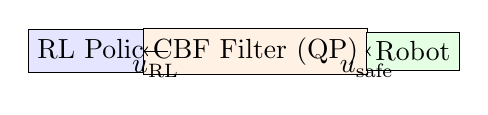
\begin{tikzpicture}[node distance=2cm, auto]
    \node[draw, rectangle, fill=blue!10] (rl) {RL Policy};
    \node[draw, rectangle, fill=orange!10, right of=rl] (cbf) {CBF Filter (QP)};
    \node[draw, rectangle, fill=green!10, right of=cbf] (robot) {Robot};
    \draw[->] (rl) -- node {$u_{\text{RL}}$} (cbf);
    \draw[->] (cbf) -- node {$u_{\text{safe}}$} (robot);
\end{tikzpicture}
\end{center}

\subsection{QP Formulation}

After RL proposes action $u_{\text{RL}}$, solve:
\begin{equation}
    \begin{aligned}
        \min_{u} \quad & \|u - u_{\text{RL}}\|^2 \\
        \text{s.t.} \quad & \nabla h_w \cdot f(x,u) + \alpha(h_w(x)) \geq \epsilon \\
        & \nabla h_o \cdot f(x,u) + \alpha(h_o(x)) \geq \epsilon \\
        & \nabla h_c \cdot f(x,u) + \alpha(h_c(x)) \geq \epsilon \\
        & u \in \mathcal{U}
    \end{aligned}
\end{equation}

where:
\begin{itemize}
    \item $h_w$: Wall CBF (keeps robot inside arena)
    \item $h_o$: Obstacle CBF (avoids obstacles)
    \item $h_c$: Collision CBF (avoids opponent, unless capture)
    \item $\delta$: Slack variables for constraint relaxation
    \item $\lambda$: Weight on slack penalty
\end{itemize}

This finds the \textbf{closest safe action} to what the RL agent wanted, measured in the control norm.

\subsection{Virtual Control Point (VCP)}

For nonholonomic robots with dynamics:
\begin{align}
    \dot{x} &= v \cos(\theta) \\
    \dot{y} &= v \sin(\theta) \\
    \dot{\theta} &= \omega
\end{align}

The position $(x,y)$ has \textbf{relative degree 2} with respect to $\omega$ (control appears after two differentiations), while $\theta$ has relative degree 1. This \textbf{mixed relative degree} makes standard CBFs fail.

\textbf{VCP Solution:} Define a point at distance $d$ ahead of the robot:
\begin{equation}
    x_{\text{vcp}} = x + d \cos(\theta), \quad y_{\text{vcp}} = y + d \sin(\theta)
\end{equation}

The VCP velocity is:
\begin{equation}
    \dot{x}_{\text{vcp}} = v \cos(\theta) - d \omega \sin(\theta), \quad \dot{y}_{\text{vcp}} = v \sin(\theta) + d \omega \cos(\theta)
\end{equation}

Now $\omega$ appears directly (relative degree 1), enabling steering-based safety.

\subsection{3-Tier Infeasibility Handling}

Sometimes constraints conflict (no safe action exists). We handle this hierarchically:
\begin{enumerate}
    \item \textbf{Tier 1:} Backup controller --- emergency stop + reverse
    \item \textbf{Tier 2:} Hierarchical relaxation --- drop least critical constraint
    \item \textbf{Tier 3:} SVM classifier --- predict infeasibility and take preemptive action
\end{enumerate}

\begin{warningbox}
\textbf{Infeasibility means danger:} If the QP is infeasible, there is no control input that satisfies all safety constraints simultaneously. This typically occurs near corners or when multiple obstacles surround the robot.
\end{warningbox}

\subsection{Why Post-Hoc (Not End-to-End)}

We initially tried BarrierNet --- end-to-end differentiable safety. It achieved only 2\% capture vs 100\% baseline.

\textbf{Root cause analysis:} Let $\rho$ be the QP intervention rate (fraction of steps where $u_{\text{safe}} \neq u_{\text{RL}}$). For BarrierNet, $\rho = 87.5\%$. The agent's gradient:
\begin{equation}
    \nabla_\phi J \approx (1-\rho) \nabla_\phi J_{\text{RL}} + \rho \nabla_\phi J_{\text{QP}}
\end{equation}

When $\rho \approx 0.875$, the RL gradient is dominated by the QP gradient, which does not improve task performance.

\begin{decisionbox}
\textbf{Decision:} Abandon end-to-end safety. Use post-hoc filter instead:
\begin{equation}
    \pi_{\text{deploy}}(s) = \text{QP}(\pi_{\text{RL}}(s), s)
\end{equation}

This separates exploration (RL training) from safety (deployment filter), allowing free exploration during training while maintaining hard guarantees at test time.
\end{decisionbox}

\chapter{The Decision Trail: How We Got Here}
\label{chap:decisions}

\section{The Big Picture}

This project did not start with the current configuration. It evolved through \textbf{86 experimental sessions} over 2.5 months. This chapter documents the key decision points --- the failures, discoveries, and pivots that shaped the final approach.

\section{The Algorithm Choice (SP1--SP11)}

\subsection{PPO vs SAC}
\textbf{Initial assumption:} PPO is the standard for continuous control.

\textbf{Reality:} On our task, PPO stalled at 0--5\% capture rate. SAC reached 30--40\% at the same step count.

\textbf{Why?} SAC's maximum entropy objective promotes exploration, which is critical when the evader constantly adapts. PPO's on-policy nature cannot keep up with a changing opponent.

\textbf{Decision D1 (2026-03-02):} Use SAC for all subsequent experiments.

\subsection{Entropy Coefficient}
\textbf{Initial assumption:} Auto-tune entropy coefficient for optimal exploration.

\textbf{Reality:} Auto-entropy caused collapse --- capture rate dropped from 24\% to 6\%.

\textbf{Why?} The entropy scheduler decreased $\alpha$ too aggressively, causing premature convergence to suboptimal policies.

\textbf{Decision D2 (2026-03-03):} Fix ent\_coef = 0.03. Never auto-tune.

\section{The Speed Ratio Saga (SP4--SP7)}

\subsection{Equal Speed (1.0x)}
\textbf{Hypothesis:} Fair game --- both agents same speed.

\textbf{Result:} Degenerate behavior. The evader learns to hide behind obstacles and barely move. No real pursuit-evasion dynamics emerge.

\subsection{Evader Advantage (1.2x)}
\textbf{Hypothesis:} Give evader 20\% speed advantage.

\textbf{Result:} Much better! Evader can escape, pursuer must develop real strategies. CR held at 35--50\%.

\subsection{Back to Equal Speed}
\textbf{Problem:} With partial observability, equal speed is actually viable because the evader can exploit blind spots. The PO itself creates enough challenge.

\textbf{Decision D5 (2026-03-02):} Return to equal speed (1.0x) but with partial observability.

\section{The Sensing Saga (SP12--SP13)}

\subsection{3m Omnidirectional (SP12)}
\textbf{Hypothesis:} Small sensing radius + masking curriculum works.

\textbf{Result:} \textbf{Catastrophic failure.} 8 runs, all failed.
\begin{itemize}
    \item 3m radius covers only 2.8\% of a $20 \times 20$m arena
    \item Agents spend most of the episode blind
    \item Mean peak CR: 0.48, mean final: 0.29
\end{itemize}

\textbf{Decision D17 (2026-03-09):} Abandon 3m radius.

\subsection{FOV 90$^\circ$ + 8m Range (SP13)}
\textbf{Hypothesis:} Directional sensing with longer range.

\textbf{Result:} \textbf{Breakthrough!}
\begin{itemize}
    \item SP13a (no obstacles): Peak 0.97 CR at full PO
    \item SP13j (alt-freeze, thr=0.8): Best self-play at CR=0.73
    \item Discovered asymmetric observations + alternate freeze at thr=0.8 is the winning formula
\end{itemize}

\textbf{Decision D18 (2026-03-09):} FOV 90$^\circ$/8m is the primary sensing config.

\section{The Freeze Saga (SP14--SP17)}

\subsection{No Freeze (SP14)}
\textbf{Hypothesis:} Pure simultaneous training works.

\textbf{Result:} Complete collapse within 2M steps.

\textbf{Decision:} Alternating freeze is \textbf{necessary}.

\subsection{Threshold Tuning (SP15)}
\textbf{Discovery:} Threshold 0.8 is unreachable. Zero switches in 10 runs.

\textbf{Why?} Under full PO, pursuer peaks at $\sim$0.75 against a static evader. It can never reach 0.8.

\textbf{Decision D21 (2026-03-16):} Use threshold 0.65 --- reachable but not trivial.

\subsection{Forced Switching (SP16)}
\textbf{Hypothesis:} Forced switch at 3M steps sustains co-evolution.

\textbf{Result:} SP16e ran 23M steps without collapse --- our best result.

\textbf{But:} Only 4 of 8 seeds converged. s42 and s44 collapsed early.

\subsection{Periodic Forced Switch (SP17)}
\textbf{Hypothesis:} Switch every 2M steps (not just once at 3M).

\textbf{Result:} SP17b s48/s49 both converged to CR$\approx$0.51--0.52. The 2M interval is superior.

\textbf{Decision D32 (2026-05-01):} 2M forced switch is the paper configuration.

\section{Failed Experiments (Documented, Not Hidden)}

\subsection{BarrierNet (Phase 2.5)}
\textbf{Goal:} End-to-end differentiable safety via differentiable QP layer.

\textbf{Result:} 2\% capture rate vs 100\% baseline.

\textbf{Root cause:} 87.5\% QP intervention rate blocked exploration. The agent could never learn because its actions were constantly overridden.

\textbf{Lesson:} Safety and exploration are fundamentally in tension. Post-hoc filter is the practical solution.

\subsection{BiMDN Belief Encoder}
\textbf{Goal:} Encode opponent position belief using Bidirectional Mixture Density Network.

\textbf{Result:} Failed Gate 1 --- could not predict opponent position when out of FOV.

\textbf{Why?} The belief encoder had no useful input when the opponent was completely unobserved.

\textbf{Lesson:} Belief encoding is hard without motion models or temporal consistency.

\subsection{RecurrentPPO (LSTM)}
\textbf{Goal:} Use LSTM to handle temporal partial observability.

\textbf{Result:} 0--2\% across 6 variants.

\textbf{Why?} LSTM policies are much harder to train. The additional complexity overwhelmed the already-difficult self-play task.

\subsection{EWC (Elastic Weight Consolidation)}
\textbf{Goal:} Prevent catastrophic forgetting when switching roles.

\textbf{Result:} No effect.

\textbf{Why?} EWC only helps if there are actual role switches. With threshold 0.8 (unreachable), there were almost no switches. EWC had nothing to protect against.

%%%%%%%%%%%%%%%%%%%%%%%%%%%%%%%%%%%%%%%%%%%%%%%%%%%%%%%%%%%%%%%%%%%%%%%%%%%%%%%%
\chapter{Experimental History}
\label{chap:experiments}

\section{Chronology}

\begin{longtable}{@{}llllp{4cm}@{}}
\toprule
\textbf{Series} \& \textbf{Dates} \& \textbf{Focus} \& \textbf{Key Finding} \& \textbf{Outcome} \\
\midrule
\endfirsthead
\multicolumn{5}{c}{\textit{Continued from previous page}} \\
\toprule
\textbf{Series} \& \textbf{Dates} \& \textbf{Focus} \& \textbf{Key Finding} \& \textbf{Outcome} \\
\midrule
\endhead
\bottomrule
\endfoot
SP1--SP10 \& Feb--Mar \& Algorithm setup \& SAC beats PPO \& Established SAC \\
SP11 \& Mar 1 \& SAC freeze/unfreeze \& ent=0.03 fixed \& Finalized hyperparams \\
SP12 \& Mar 6 \& Masking curriculum (3m) \& 3m radius too small (2.8\% coverage) \& All 8 failed \\
SP13 \& Mar 8--10 \& FOV 90$^\circ$/8m \& Asymmetric + alt-freeze wins \& Best: CR=0.82 \\
SP14 \& Mar 10 \& Pure self-play \& Complete collapse \& Freeze necessary \\
SP15 \& Mar 15--16 \& Vis reward + thresholds \& Vis reward mandatory (6$\times$ improvement) \& thr=0.65 works \\
SP16 \& Mar 16--Apr 28 \& Forced switch + EWC \& 4 converged, EWC useless \& 23M stable run \\
SP17 \& Apr 29--May \& Refined SP16 + search \& 2M switch better than 3M \& Converging \\
\bottomrule
\end{longtable}

\section{SP13: The Breakthrough Series}

SP13 was our most extensive series (22 runs) and produced the key discoveries:

\begin{table}[h]
\centering
\caption{SP13 Key Results}
\begin{tabular}{@{}llll@{}}
\toprule
\textbf{Run} \& \textbf{Config} \& \textbf{Peak CR} \& \textbf{Notes} \\
\midrule
SP13a s42 \& FOV, no obs, freeze evader \& 0.97 \& Upper bound \\
SP13j s43 \& Alt-freeze thr=0.8, obs \& 0.73 \& Best self-play \\
SP13l s43 \& Asymmetric + alt-freeze \& 0.89 \& Still climbing when killed \\
\bottomrule
\end{tabular}
\end{table}

\textbf{Key discovery:} Alternate freeze at threshold 0.8 + asymmetric observations is the winning formula for self-play.

\section{SP16: The Stability Series}

SP16 tested forced switching and EWC:

\begin{table}[h]
\centering
\caption{SP16 Results (8 seeds)}
\begin{tabular}{@{}llll@{}}
\toprule
\textbf{Seed} \& \textbf{Config} \& \textbf{Final CR} \& \textbf{Status} \\
\midrule
s43 \& vis=0.1, thr=0.65, force@3M \& 0.52 \& Converged \\
s44 \& vis=0.1, thr=0.65, force@3M \& 0.48 \& Converged \\
s45 \& vis=0.2, thr=0.65, force@3M \& 0.52 \& Converged \\
s46 \& vis=0.2, thr=0.55, force@3M \& 0.48 \& Converged \\
\bottomrule
\end{tabular}
\end{table}

SP16e (not in table above) was the champion: 23M steps, 76 phases, no collapse.

\section{SP17: Current Best}

\textbf{Changes from SP16:}
\begin{itemize}
    \item Periodic forced switch every 2M steps (not just once)
    \item Search staleness reward enabled ($w_{\text{search}} = 0.0001$)
    \item Visibility reward at $w_{\text{vis}} = 0.2$
    \item 5-seed validation cohort
\end{itemize}

\textbf{Current status:}
\begin{itemize}
    \item s48 (seed 48): CR = 0.51, converged at M2550
    \item s49 (seed 49): CR = 0.52, converged at M2700
    \item s50/s51: Running (launched May 1)
\end{itemize}

%%%%%%%%%%%%%%%%%%%%%%%%%%%%%%%%%%%%%%%%%%%%%%%%%%%%%%%%%%%%%%%%%%%%%%%%%%%%%%%%
\chapter{Training Infrastructure}
\label{chap:infrastructure}

\section{The Training Script}

\texttt{scripts/train\_amsdrl.py} is the main entry point (557 lines). It:

\begin{enumerate}
    \item Parses 80+ CLI arguments (environment, rewards, self-play, safety, curriculum)
    \item Instantiates \texttt{AMSDRLSelfPlay} protocol
    \item Runs training loop
    \item Saves checkpoints, history JSON, convergence analysis
\end{enumerate}

\section{The AMS-DRL Protocol}

\texttt{training/amsdrl.py} implements the full protocol:

\subsection{Phase S0: Initialization}
\begin{itemize}
    \item \textbf{Warm-seed:} Load pre-trained models (if available)
    \item \textbf{Cold-start:} Pre-train evader with \texttt{NavigationEnv} for goal-reaching + flee behavior
    \item Evaluate baseline metrics
\end{itemize}

\subsection{Micro-Phase Loop}
\begin{lstlisting}[language=Python]
for phase in range(max_phases):
    # Train active agent for 2048 steps
    # Opponent frozen (loaded from pool or current best)
    # Evaluate every 150 micro-phases
    # Check for collapse, forced switch, convergence
\end{lstlisting}

\subsection{Convergence Detection}
\begin{equation}
    |\text{CR} - (1 - \text{CR})| < \eta \quad \text{for 5 consecutive evals}
\end{equation}
where $\eta = 0.10$ (default). This means capture rate stays within $[0.45, 0.55]$.

\section{Checkpoint Management}

\begin{itemize}
    \item \textbf{Milestone checkpoints:} Saved every N phases
    \item \textbf{Best-model checkpoint:} Updated whenever eval improves
    \item \textbf{History JSON:} Contains full training log (capture rate, escape rate, mean episode length, frozen role, etc.)
    \item \textbf{TensorBoard:} Live training metrics
\end{itemize}

\section{Configuration with Hydra}

All experiments are configured via Hydra:
\begin{lstlisting}[language=bash]
python scripts/train_amsdrl.py \
  algorithm=sac \
  env=pe_fov \
  experiment=sp17b \
  self_play=alternate_freeze
\end{lstlisting}

This enables reproducible, versioned configurations.

%%%%%%%%%%%%%%%%%%%%%%%%%%%%%%%%%%%%%%%%%%%%%%%%%%%%%%%%%%%%%%%%%%%%%%%%%%%%%%%%
\chapter{Behavioral Analysis}
\label{chap:behavior}

\section{What Emerges from Training?}

When policies converge, they exhibit sophisticated behaviors that were never explicitly programmed:

\subsection{Pursuer Strategies}
\begin{itemize}
    \item \textbf{Cornering:} Drives evader toward arena boundaries where escape is limited
    \item \textbf{Obstacle-aware paths:} Takes curved trajectories around obstacles to maintain LOS
    \item \textbf{FOV exploitation:} Positions itself to maximize visible area
    \item \textbf{Cut-off:} Predicts evader trajectory and intercepts
\end{itemize}

\subsection{Evader Strategies}
\begin{itemize}
    \item \textbf{Boundary hugging:} Stays near walls to limit pursuer approach angles
    \item \textbf{Obstacle blocking:} Places obstacles between itself and pursuer
    \item \textbf{FOV exploitation:} Stays outside pursuer's FOV wedge
    \item \textbf{Feints:} Makes sudden direction changes to break pursuit
\end{itemize}

\section{Visualization Pipeline}

We generate trajectory visualizations using GPU-accelerated rendering:
\begin{itemize}
    \item \textbf{CPU rendering:} $\sim$1.8 steps/sec (11+ min per episode)
    \item \textbf{GPU rendering:} $\sim$60 steps/sec (20 sec per episode) --- \textbf{60$\times$ speedup}
\end{itemize}

\section{Deterministic vs Stochastic Policies}

\begin{itemize}
    \item \textbf{Training:} Stochastic policies (sample from action distribution)
    \item \textbf{Evaluation:} Deterministic policies (mean action)
    \item \textbf{Behavioral analysis:} Deterministic policies show cleaner, more interpretable strategies
\end{itemize}

\begin{warningbox}
\textbf{Important:} Capture rate in visualization (deterministic) is often higher than training eval (stochastic). For s43 M2550: viz CR = 78\%, training eval CR = 54\%. Always report the training eval as the ground truth.
\end{warningbox}

%%%%%%%%%%%%%%%%%%%%%%%%%%%%%%%%%%%%%%%%%%%%%%%%%%%%%%%%%%%%%%%%%%%%%%%%%%%%%%%%
\chapter{Current Status and CoRL Paper Plan}
\label{chap:corl}

\section{What We Have}

\subsection{Completed Components}
\begin{itemize}
    \item Full simulation environment with realistic physics (700+ tests)
    \item FOV-based partial observability with masking curriculum
    \item Self-play framework with opponent pool, PFSP, collapse recovery
    \item Forced periodic switching mechanism
    \item Visibility reward and search staleness reward
    \item CBF safety filter (post-hoc, proven effective)
    \item 86 experimental sessions of iteration and discovery
\end{itemize}

\subsection{Working Results}
\begin{itemize}
    \item 2 converged seeds at CR $\approx$ 0.51--0.52 (s48, s49)
    \item Sustained co-evolution past 10M+ steps
    \item Emergent strategies: cornering, obstacle use, FOV exploitation
    \item Ablation evidence: visibility reward gives 6$\times$ improvement
\end{itemize}

\section{What's In Progress}

\subsection{Experiments Running (May 1)}
\begin{itemize}
    \item s50, s51 (convergence cohort on niro-2)
    \item ABL-1 (no vis reward), ABL-2 (no forced switch) on niro-1
\end{itemize}

\subsection{Still Needed}
\begin{itemize}
    \item 1 more convergence seed (s52)
    \item 2 more ablations (no search, no curriculum)
    \item 2 baselines (full obs, greedy)
    \item Behavior analysis on all converged models
    \item Publication-quality figures
\end{itemize}

\section{Paper Contributions}

\begin{enumerate}
    \item \textbf{Visibility reward} stabilizes pursuer learning under FOV partial observability
    \item \textbf{Forced periodic switching} prevents freeze-sticking and sustains co-evolution past 10M+ steps
    \item \textbf{Search staleness reward} teaches systematic area coverage when evader is out of FOV
    \item \textbf{Multi-seed validation} showing consistent NE convergence under realistic sensing constraints
\end{enumerate}

\section{Timeline}

\begin{table}[h]
\centering
\caption{CoRL 2026 Timeline}
\begin{tabular}{@{}lll@{}}
\toprule
\textbf{Date} \& \textbf{Milestone} \& \textbf{Status} \\
\midrule
May 1 \& All experiments launched \& Done \\
May 7 \& First evals from new seeds \& Pending \\
May 14 \& 3+ seeds converged, ablations complete \& Pending \\
May 21 \& Full paper draft \& Pending \\
May 28 \& Submit to CoRL \& Pending \\
\bottomrule
\end{tabular}
\end{table}

\begin{infobox}
\textbf{Backup plan:} If CoRL submission is not ready by May 28, use reviewer feedback to strengthen an ICRA 2027 submission (deadline $\sim$September 2026).
\end{infobox}

%%%%%%%%%%%%%%%%%%%%%%%%%%%%%%%%%%%%%%%%%%%%%%%%%%%%%%%%%%%%%%%%%%%%%%%%%%%%%%%%
\chapter{Glossary}
\label{chap:glossary}

\begin{description}
    \item[AMS-DRL] Adversarial Multi-Stage Deep RL --- our self-play protocol
    \item[CBF] Control Barrier Function --- mathematical tool for safety guarantees
    \item[CR] Capture Rate --- fraction of episodes where pursuer catches evader
    \item[DCBF] Discrete-time Control Barrier Function --- CBF for discrete systems
    \item[EWC] Elastic Weight Consolidation --- regularization against forgetting
    \item[FOV] Field of View --- angular range an agent can see (\SI{90}{\degree} in our config)
    \item[LOS] Line of Sight --- direct visibility without occlusion
    \item[NE] Nash Equilibrium --- stable strategy pair where neither can improve unilaterally
    \item[POMDP] Partially Observable Markov Decision Process
    \item[PO] Partial Observability
    \item[PFSP] Prioritized Fictitious Self-Play --- opponent sampling strategy
    \item[QP] Quadratic Program --- optimization problem solved for safety filter
    \item[SAC] Soft Actor-Critic --- our RL algorithm
    \item[SB3] Stable Baselines3 --- RL library we use
    \item[SR] Success Rate --- same as capture rate
    \item[VCP] Virtual Control Point --- point ahead of robot for CBF constraints
    \item[BiMDN] Bidirectional Mixture Density Network --- belief encoder (abandoned)
\end{description}

\end{document}
